%% IEEE Conference Paper - revised v2
%% Fast PUF-Based Four-Phase Authentication for UAV Swarms
%% Compile: pdflatex uav_puf_conference.tex   (run twice for cross-refs)

\documentclass[conference,a4paper,10pt]{IEEEtran}
\IEEEoverridecommandlockouts

\usepackage{cite}
\usepackage{amsmath,amssymb,amsfonts}
\usepackage{algorithm,algorithmic}
\usepackage{graphicx}
\usepackage{textcomp}
\usepackage{xcolor}
\usepackage{booktabs}
\usepackage{array}
\usepackage{multirow}
\usepackage{url}
\usepackage{hyperref}
\usepackage{balance}
\usepackage{pifont}
\usepackage{pgfplots}
\pgfplotsset{compat=1.18}

\newcommand{\xmark}{\ding{55}}
\newcommand{\cmark}{\checkmark}

\hypersetup{
  colorlinks=true,
  linkcolor=blue!50!black,
  citecolor=blue!50!black,
  urlcolor=blue!60!black,
  pdftitle={Fast PUF-Based Four-Phase Authentication for UAV Swarms},
  pdfauthor={Md Ziyad Hussain and Rakesh Matam}
}

\setlength{\textfloatsep}{6pt plus 1pt minus 1pt}
\setlength{\dbltextfloatsep}{6pt plus 1pt minus 1pt}

\begin{document}

\title{Fast PUF-Based Four-Phase Authentication for\\
UAV Swarms: An OMNeT++ Evaluation with\\
SHA3-256 and SPONGENT-160 Hash Modes}

\author{%
\IEEEauthorblockN{Md Ziyad Hussain}
\IEEEauthorblockA{\textit{Dept.\ of Computer Science and Engineering}\\
\textit{Indian Institute of Information Technology Guwahati}\\
Bongora, Assam 781015, India \\
ziyad.hussain23b@iiitg.ac.in}
\and
\IEEEauthorblockN{Rakesh Matam}
\IEEEauthorblockA{\textit{Dept.\ of Computer Science and Engineering}\\
\textit{Indian Institute of Information Technology Guwahati}\\
Bongora, Assam 781015, India \\
rakesh@iiitg.ac.in}
}

\maketitle

% ========================================================================
\begin{abstract}
Unmanned Aerial Vehicle (UAV) swarms require fast, lightweight, and
capture-resilient authentication for real-time coordination.
Public-key alternatives (RSA-2048, ECC-256) add millisecond-scale
handshake overhead and rely on private keys stored in non-volatile
memory---keys that are exposed when a UAV is physically captured.
We present a four-phase Physical Unclonable Function (PUF)-based
authentication protocol covering: enrollment with a BCH(255,131,18)
fuzzy extractor; UAV--Ground Station mutual authentication; direct
full-mesh UAV--UAV peer authentication via a swarm-wide credential
issued in Phase~2; and symmetric session-key establishment with
optional Curve25519 forward secrecy. The protocol uses only hash,
XOR, and PUF primitives, and is fully implemented in OMNeT++~6.3 for
a ten-UAV stadium-surveillance scenario ($500{\times}300$\,m). We
characterize two hash primitives back-to-back: SHA3-256 truncated to
160~bits (via OpenSSL EVP) and a SPONGENT-160-style lightweight
sponge. Measured end-to-end Phase~2 latency is
\textbf{0.699~ms} (SHA3) and \textbf{14.044~ms} (SPONGENT);
Phase~3 per-pair latency is \textbf{0.476~ms} and \textbf{14.535~ms};
communication overhead is 175\,B and 104\,B per phase, with
$100\%$ authentication success across all ten UAV--GS exchanges and
$45$ peer pairs. Per-message timing breakdowns localize cost to PUF
evaluation, BCH decoding, and hash operations, enabling a synthesis-
based projection in which the SHA3--SPONGENT gap collapses from
$20$--$30\times$ in software to $2$--$5\times$ on FPGA/ASIC. Our
SHA3 mode is $11$--$21\times$ faster than RSA/ECC baselines while
removing the stored-key attack surface entirely.
\end{abstract}

\begin{IEEEkeywords}
UAV swarm authentication, Physical Unclonable Function, PUF,
SPONGENT, SHA3, lightweight cryptography, fuzzy extractor, BCH error
correction, OMNeT++, peer-to-peer authentication.
\end{IEEEkeywords}


% ========================================================================
\section{Introduction}
\label{sec:intro}

\IEEEPARstart{U}{nmanned} Aerial Vehicles (UAVs) are increasingly
deployed as cooperating swarms for stadium surveillance, border
patrol, search-and-rescue, agricultural sensing, and disaster
response~\cite{securing_uav_fanet}. A common operational pattern---
ten or more drones cooperatively covering a fixed perimeter---demands
sub-millisecond mutual authentication between each UAV and a Ground
Station (GS) and, increasingly, between UAV pairs without GS
mediation when relay latency is unacceptable or the GS link is
intermittent.

Conventional authentication options are poorly suited to this regime.
\textbf{RSA-2048 PKI} requires $8$--$15$~ms per signature verification
on an ARM Cortex-A72~\cite{puf_lightweight_uav}, growing to nearly
a second for full-mesh authentication of a ten-UAV swarm and adding
$256$--$512$\,B certificates per exchange. \textbf{ECC-256}
~\cite{peer2peer_auth} halves the latency but still depends on
private keys held in non-volatile memory---recoverable from a
captured UAV by cold-boot or side-channel attacks. \textbf{Pre-shared
keys (PSK)} reach sub-millisecond latency but compromise the entire
swarm if any device is captured, and require $O(N^2)$ pairwise keys.

\textbf{Physical Unclonable Functions (PUFs)} provide a hardware root
of trust without any stored key: the response to a challenge is
produced by the silicon's manufacturing variations, is unique to each
device, and cannot be cloned even by the
manufacturer~\cite{puf_overview}. A PUF-based protocol shifts the
attack surface from extractable memory to physical capture-and-clone
attacks that today's adversaries cannot mount. The challenge is that
PUF responses are noisy ($3$--$10\%$ bit-flip rate); a BCH-based
fuzzy extractor~\cite{bch_puf_extraction, helper_data_masking}
recovers the enrollment-time response despite environmental drift.

\subsection*{Contributions}
\begin{enumerate}
\item A complete four-phase PUF-based authentication protocol
  covering enrollment, UAV--GS authentication, GS-less full-mesh
  UAV--UAV peer authentication, and session-key derivation. Phase~3
  avoids GS round-trips by using a swarm-wide credential issued in
  Phase~2 as the shared root of trust.
\item An OMNeT++~6.3 reference implementation with a composite
  link-delay model, a $128$-stage Arbiter PUF simulator, a
  from-scratch BCH(255,131,18) fuzzy extractor with Berlekamp-Massey
  decoding, and a dual-mode hash wrapper with per-mode timing
  accumulators.
\item End-to-end performance characterization across $10$ UAV--GS
  authentications and $45$ peer pairs, with per-message latency
  decomposition into UAV-side, GS-side, and network components.
\item A synthesis-based software-vs.-hardware projection showing
  that SPONGENT's software cost becomes negligible on FPGA/ASIC,
  bringing total ten-UAV swarm authentication to $\sim 29$\,ms
  regardless of hash mode.
\end{enumerate}

The remainder of the paper covers related work
(\S\ref{sec:related}), protocol (\S\ref{sec:protocol}),
implementation (\S\ref{sec:implementation}), evaluation
(\S\ref{sec:evaluation}), security and discussion
(\S\ref{sec:security}), and conclusions (\S\ref{sec:conclusion}).


% ========================================================================
\section{Related Work}
\label{sec:related}

\textbf{PUF-based UAV authentication.}
Gope and Sikdar~\cite{puf_lightweight_uav} proposed a hash/XOR-only
PUF authentication for UAV networks, reporting $10$--$50$\,ms
latency on a Raspberry Pi~4B, but addressing only UAV-to-GS
authentication. Li \textit{et al.}~\cite{puf_uav_cross_domain}
extended PUF authentication to cross-domain emergency-rescue UAVs at
the cost of $640$\,B overhead and $45$--$80$\,ms latency on embedded
ARM. Khan \textit{et al.}~\cite{puf_6g_uav} combined PUF with
biometrics for $6$G UAV networks; their formal real-or-random (ROR)
model security analysis provides a strong verification framework.
Dey and Hossain~\cite{puf_mitm_dos} proposed MITM- and DoS-resistant
PUF authentication via sensor-initiated registration. Xu \textit{et
al.}~\cite{arbiter_puf_iot} introduced dynamic CRP rotation to
prevent database exhaustion, which we adopt.

\textbf{Peer-to-peer authentication.}
Direct UAV--UAV authentication remains under-explored. Bera \textit{et
al.}~\cite{peer2peer_auth} achieved sub-millisecond P2P
authentication using pre-shared symmetric keys, but lacked a PUF
hardware root of trust. Banerjee \textit{et
al.}~\cite{puf_uav_security_analysis} identified vulnerabilities in
prior UAV--GS authentication schemes (impersonation, session-key
compromise, lack of forward secrecy), motivating our explicit
security analysis. To our knowledge, no prior work characterizes a
full-mesh PUF-based peer authentication scheme end-to-end in a
discrete-event network simulator with per-message timing.

\textbf{Lightweight cryptography.}
Bogdanov \textit{et al.}~\cite{spongent_original} introduced SPONGENT,
achieving $2{,}190$~gate equivalents (GE) for SPONGENT-160; the
bit-level permutation requires zero logic (only wire routing).
SHA3/Keccak~\cite{sha3_standard, keccak_team} is software-fast (
$\sim$0.4~\textmu s per call on modern x86) but requires $\sim
38{,}000$\,GE in hardware. The crossover between these two regimes
motivates our dual-mode evaluation.


% ========================================================================
\section{Proposed Protocol}
\label{sec:protocol}

\subsection{System and Threat Model}
A swarm consists of one trusted GS and $N$ UAVs. Each UAV embeds a
$128$-stage Arbiter PUF, a lightweight processor, and a wireless link.
We adopt the Dolev-Yao adversarial model~\cite{dolev_yao} augmented
with physical capture: the adversary may extract NVM but cannot clone
PUF hardware (tamper-evident probing destroys the response). Hashes
are pre-image and collision resistant; PUFs are unclonable and
unpredictable.

\textbf{Notation.} $\mathrm{TID}_i$ is the temporary identity of
UAV~$i$, $C_i^{(k)}$ the $k$-th challenge,
$R_i^{(k)}=\mathrm{PUF}_i(C_i^{(k)})$ the noisy response,
$H_i^{(k)}$ its BCH helper data, $h(\cdot)$ a $160$-bit hash,
$\oplus$ bitwise XOR, $\|$ concatenation, $T_x$ a $32$-bit timestamp,
$N_x, n_x$ random $128$-bit nonces.

\subsection{Phase 1: Secure Enrollment}
Enrollment is performed once per UAV in a physically secure facility.
For each UAV $i$ and each of $n{\ge}12$ random challenges, the GS
records $(C_i^{(k)}, R_i^{(k)})$ and computes helper data following
the fuzzy-extractor Gen construction:
\begin{equation}
H_i^{(k)} = \mathrm{BCH\_encode}(R_i^{(k)}) \oplus R_i^{(k)}.
\label{eq:gen}
\end{equation}
Under Maes' helper-data-masking analysis~\cite{helper_data_masking},
$H$ is computationally independent of $R$. After enrollment the UAV
holds only its TID; no key material of any kind is stored.

\subsection{Phase 2: UAV--GS Mutual Authentication}
Phase~2 is a four-message protocol (Alg.~\ref{alg:phase2}) executed
when a UAV joins the swarm. The UAV first authenticates itself with
a hashed nonce; the GS issues a fresh CRP challenge and its own
authenticator; the UAV evaluates its PUF, masks the response, and
returns an authentication token; the GS performs BCH correction,
verifies the token, and on success issues a swarm-wide credential
$\mathrm{Cred}$.

\begin{algorithm}[t]
\caption{Phase 2 UAV--GS Mutual Authentication}
\label{alg:phase2}
\begin{algorithmic}[1]
\STATE \textbf{UAV $\to$ GS:} $\langle \mathrm{TID}_i, T_1, N_1,\,
  h(\mathrm{TID}_i\|T_1\|N_1) \rangle$
\STATE \textbf{GS:} verify hash, look up TID, fetch
  $(C_i^{(k)}, H_i^{(k)}, R_i^{(k)})$, draw $N_2$
\STATE \textbf{GS $\to$ UAV:} $\langle C_i^{(k)}, N_2,\,
  h(\mathrm{TID}_i\|C_i^{(k)}\|N_2\|T_1) \rangle$
\STATE \textbf{UAV:} verify GS hash; $R^{\mathrm{n}} \leftarrow
  \mathrm{PUF}_i(C_i^{(k)})$
\STATE \textbf{UAV:} $R^{\mathrm{m}} \leftarrow R^{\mathrm{n}}\oplus
  h(N_2)$;\ $\mathrm{SK}_i \leftarrow
  h(R^{\mathrm{n}}\|N_1\|N_2\|T_1)$
\STATE \textbf{UAV $\to$ GS:} $\langle R^{\mathrm{m}},\,
  h(R^{\mathrm{m}}\|\mathrm{SK}_i) \rangle$
\STATE \textbf{GS:} recover $R^{\mathrm{n}}$, compute ecc
  $= H_i^{(k)}\oplus R^{\mathrm{n}}$, decode $R \leftarrow
  \mathrm{BCH\_decode}(R^{\mathrm{n}},\mathrm{ecc})$
\STATE \textbf{GS:} check $\mathrm{HD}(R, R_i^{(k)}){\le}\tau$,
  verify token, advance CRP index
\STATE \textbf{GS $\to$ UAV:} $\langle \mathrm{success},\,
  \mathrm{Cred} \rangle$
\end{algorithmic}
\end{algorithm}

\subsection{Phase 3: UAV--UAV Peer Authentication}
After Phase~2, each pair $(i,j)$ with $i{<}j$ runs a three-message
exchange using $\mathrm{Cred}$ as the shared root of trust:
\begin{align}
P_1: &\ \mathrm{UAV}_i \to \mathrm{UAV}_j:\ \langle n_i,\,
  h(i\|j\|n_i\|\mathrm{Cred}) \rangle, \\
P_2: &\ \mathrm{UAV}_j \to \mathrm{UAV}_i:\ \langle n_j,\,
  h(j\|i\|n_i\|n_j\|\mathrm{Cred}) \rangle, \\
P_3: &\ \mathrm{UAV}_i \to \mathrm{UAV}_j:\ \langle
  h(i\|j\|n_j\|\mathrm{Cred}) \rangle.
\end{align}
Both endpoints then derive
$\mathrm{SK}_{ij}=h(i\|j\|n_i\|n_j\|\mathrm{Cred})$. Possession of
$\mathrm{Cred}$ is gated by Phase~2 success---hence by PUF
possession---so $\mathrm{Cred}$ acts as a PUF-rooted shared secret.

\subsection{Phase 4: Session Key}
The keys derived in Phases~2 and~3 ($\mathrm{SK}_i$ and
$\mathrm{SK}_{ij}$) are the established session keys.
For applications requiring perfect forward secrecy, Phase~4 can be
extended with an ephemeral Curve25519 exchange folded into
$\mathrm{SK}_{ij}$~\cite{puf_key_exchange}; the reference
implementation gates this on a compile-time \texttt{USE\_SODIUM} flag.


% ========================================================================
\section{OMNeT++ Implementation}
\label{sec:implementation}

\subsection{Module Architecture}
The simulation defines three OMNeT++ simple modules:
\texttt{UAVNode} (Phase~2 client, Phase~3 initiator/responder),
\texttt{GroundStation} (enrollment database, Phase~2 verifier, BCH
decoder, credential issuer), and \texttt{NetworkController}
(lifecycle). Inter-module communication uses
\texttt{sendDirect()} with a composite delay model:
\begin{equation}
d = \frac{\mathrm{dist}}{c}
  + \frac{8\,L}{r}
  + d_{\mathrm{proc}}
  + d_{\mathrm{jitter}},
\label{eq:delay}
\end{equation}
where $L$ is payload bytes, $r{=}6$~Mbps (802.11a baseline),
$d_{\mathrm{proc}}{=}0.1$~ms is the mean processing delay, and
$d_{\mathrm{jitter}}{\sim}|\mathcal{N}(0, 0.02^2)|$~ms is a
half-Gaussian queue jitter. MAC-layer contention is not modeled; the
reported network delay is a lower bound on real $802.11$, but the
relative comparisons between hash modes are unaffected.

\subsection{Cryptographic Primitives}
\textbf{PUF.} A $128$-stage Arbiter-style simulator. Each challenge
is hashed (FNV-1a) into a device-seeded \texttt{mt19937} state, $128$
response bits are generated, and a Bernoulli$(0.03)$ noise channel
flips bits uniformly. Inter-chip Hamming distance is empirically
$45$--$55\%$ and intra-chip $\le 5\%$, consistent with the Arbiter
PUF literature~\cite{arbiter_puf_iot}.

\textbf{BCH(255,131,18).} A from-scratch GF$(2^8)$ codec with
Berlekamp-Massey error-locator polynomial and Chien search,
correcting up to $t{=}18$ bit errors. With $128$-bit responses at
$3\%$ BER, the expected error count per evaluation is
$128{\cdot}0.03{=}3.84$, giving a $\sim 4.7\times$ margin to the BCH
correction capacity. The probability of exceeding $18$ errors in a
$128$-bit block is $<\!10^{-15}$ by Chernoff bound, so steady-state
decoding failure is effectively impossible.

\textbf{SHA3-256.} Via OpenSSL's EVP API (\texttt{EVP\_sha3\_256}),
truncated to $160$~bits. A warm-up call in each module's
\texttt{initialize()} absorbs the $\sim$2.8~ms cold-start cost so
that per-call timing reflects steady state ($\sim$0.4~\textmu s).

\textbf{SPONGENT-160.} A lightweight sponge construction with the
PRESENT-type $4$-bit S-box, rate $r{=}16$, capacity $c{=}144$,
$80$ rounds, and a compact bit-permutation suitable for relative
timing characterization\footnote{The full SPONGENT-160 bit-permutation
is trivial in hardware (deterministic wire routing) but
software-unfriendly. Our implementation preserves the round count,
S-box, rate, capacity, and order-of-magnitude software cost; a
full-spec evaluation is left as future work.}. Per-call software cost
on the test platform is $\sim$890~\textmu s.

\textbf{Hash wrapper.} A runtime-mode-selectable abstraction
maintaining per-mode timing accumulators
(\texttt{sha3TimeMs}, \texttt{spongentTimeMs}), enabling back-to-back
comparison without code duplication.

\subsection{Stadium Scenario}
The reference scenario places ten UAVs around the perimeter of a
$500{\times}300$~m stadium with the GS at $(275, 175)$~m.
Phase~2 start times are staggered by $0.5$~s. Phase~3 full-mesh
authentication is launched $10$~s after each UAV completes Phase~2,
yielding $45$ peer pairs ($\binom{10}{2}$). Simulation duration is
$120$~s.

\subsection{Validation: PUF Quality Metrics}
\label{sec:puf_quality}
We validate the PUF simulator against the two standard metrics
before exercising it in the protocol. With $1{,}000$ distinct
$(\mathrm{seed}, C)$ pairs evaluated on each simulated device,
\emph{uniqueness} (mean inter-chip Hamming distance across $100$
devices) was $49.8\%$ with standard deviation $4.3\%$---within the
$45$--$55\%$ band expected from an ideal Arbiter
PUF~\cite{arbiter_puf_iot}. \emph{Reliability} (mean intra-chip
Hamming distance over $1{,}000$ re-evaluations of the same
challenge) was $3.0\%$, matching the Bernoulli noise rate set at
construction. The $128$-bit response space is exhausted only after
$2^{128}$ challenges, so CRP rotation handles the practical
exhaustion-prevention requirement.


% ========================================================================
\section{Evaluation}
\label{sec:evaluation}

All measurements are from the \texttt{StadiumSHA3} and
\texttt{StadiumSPONGENT} configurations, release build
(\texttt{-O3}), on an x86-64 laptop. Reported values are means over
the simulation population ($10$ UAVs for Phase~2, $45$ peer pairs
for Phase~3). Absolute values reflect software execution on this
platform; the relative ordering between hash modes carries to any
platform, while absolute values shift with processor capability or
hardware acceleration (\S\ref{sec:hwproj}).

\subsection{Phase 2 Aggregate Results}
\label{sec:p2agg}
Table~\ref{tab:phase2} reports Phase~2 end-to-end metrics over the
ten UAVs. Total compute is broken into UAV-side and GS-side
contributions because both add to wall-clock latency in this
single-CPU-per-node model.

\begin{table}[t]
\centering
\caption{Phase 2 UAV--GS authentication: aggregate results ($N{=}10$).}
\label{tab:phase2}
\begin{tabular}{@{}lrr@{}}
\toprule
\textbf{Metric} & \textbf{SHA3-256} & \textbf{SPONGENT-160} \\
\midrule
UAV-side compute (\textmu s)     & $7.2$    & $6{,}703$  \\
\quad of which hash (\textmu s)  & $3.4$    & $6{,}697$  \\
GS-side compute (\textmu s)      & $26.9$   & $6{,}676$  \\
Network delay (\textmu s)        & $664.6$  & $664.6$    \\
\midrule
\textbf{End-to-end latency} (ms) & $\mathbf{0.699}$ & $\mathbf{14.044}$ \\
Communication overhead (B)       & $175$    & $175$    \\
Authentication success rate      & $10/10$  & $10/10$  \\
\bottomrule
\end{tabular}
\end{table}

\textbf{Observations.} In SHA3 mode, compute (UAV + GS = $34.1$
\textmu s) is $4.9\%$ of latency; network delay dominates at $95\%$.
In SPONGENT mode, compute ($13{,}379$~\textmu s) is $95\%$ of
latency. Network delay is identical between modes because message
sizes are identical---hash mode affects only on-device compute. All
ten Phase~2 exchanges succeed.

\subsection{Phase 2 Per-Message Breakdown}
\label{sec:p2bd}
Table~\ref{tab:phase2_break} decomposes the four-message exchange
step by step. Per-step values are means over the ten UAVs and sum
exactly to the aggregate totals in Table~\ref{tab:phase2}.

\begin{table}[t]
\centering
\caption{Phase 2 per-message timing breakdown (\textmu s).
``GS'' includes BCH decoding inside step M3.}
\label{tab:phase2_break}
\begin{tabular}{@{}p{4.5cm}rr@{}}
\toprule
\textbf{Step} & \textbf{SHA3} & \textbf{SPONGENT} \\
\midrule
M1: UAV computes $\alpha_1$ (hash)        & $1.5$   & $1{,}094$ \\
M1: Network transit                       & $172.9$ & $172.9$ \\
M1: GS verifies hash, lookup CRP          & $2.5$   & $2{,}606$ \\
M2: Network transit                       & $185.0$ & $185.0$ \\
M2: UAV verifies GS hash                  & $1.0$   & $1{,}499$ \\
M2: UAV PUF evaluation                    & $2.5$   & $3.2$ \\
M3: UAV crypto (mask + SK + token)        & $2.2$   & $4{,}107$ \\
M3: Network transit                       & $169.1$ & $169.1$ \\
M3: GS unmask + BCH decode + verify       & $24.3$  & $4{,}070$ \\
M4: Network transit                       & $137.6$ & $137.6$ \\
M4: UAV finalizes                         & $0.03$  & $0.05$ \\
\midrule
\textbf{Total UAV compute}                & \textbf{7.2} & \textbf{6{,}703} \\
\textbf{Total GS compute}                 & \textbf{26.9} & \textbf{6{,}676} \\
\textbf{Total network}                    & \textbf{664.6} & \textbf{664.6} \\
\textbf{End-to-end latency}               & \textbf{698.7} & \textbf{14{,}043.7} \\
\bottomrule
\end{tabular}
\end{table}

In SHA3 mode, BCH decoding ($\sim 22$~\textmu s, included within the
GS M3 step) is the dominant non-hash cost. In SPONGENT mode every
hash-bearing step inflates by roughly three orders of magnitude; the
M3 step in particular requires three hash calls on each side
(mask, session key, token), explaining its $\sim 4$~ms cost.

\subsection{Phase 3 Aggregate Results}
Phase~3 is symmetric---both endpoints are UAVs of equivalent
capability---so the timing decomposition has only four
compute/network steps in series (Table~\ref{tab:phase3}).

\begin{table}[t]
\centering
\caption{Phase 3 peer authentication: aggregate results
(mean of $45$ pairs).}
\label{tab:phase3}
\begin{tabular}{@{}lrr@{}}
\toprule
\textbf{Metric} & \textbf{SHA3-256} & \textbf{SPONGENT-160} \\
\midrule
Total compute (\textmu s)         & $9.2$    & $14{,}069$ \\
\quad of which hash (\textmu s)   & $6.3$    & $14{,}062$ \\
Network delay (\textmu s)         & $466.8$  & $466.8$ \\
\midrule
\textbf{End-to-end latency} (ms)  & $\mathbf{0.476}$ & $\mathbf{14.535}$ \\
Communication overhead (B)        & $104$    & $104$ \\
Authentication success rate       & $45/45$  & $45/45$ \\
\bottomrule
\end{tabular}
\end{table}

Phase~3 SHA3 is faster than Phase~2 SHA3 ($0.476$~ms vs.\ $0.699$~ms)
because there are three messages instead of four, no PUF evaluation,
and no BCH decoding. Phase~3 SPONGENT ($14.535$~ms) is slightly
larger than Phase~2 SPONGENT ($14.044$~ms) because both endpoints
each perform multiple hashes (initiator: build $\tau_1$, verify
$\tau_2$, build $\tau_3$; responder: verify $\tau_1$, build $\tau_2$,
verify $\tau_3$), summing to $\sim$16 SPONGENT calls per pair.

\subsection{Phase 3 Per-Message Breakdown}
\label{sec:p3bd}
Table~\ref{tab:phase3_break} decomposes the three-message peer
exchange step by step; values sum exactly to the aggregate totals.

\begin{table}[t]
\centering
\caption{Phase 3 per-message timing breakdown (\textmu s, mean of
$45$ pairs). Initiator denoted $\mathrm{UAV}_i$, responder
$\mathrm{UAV}_j$.}
\label{tab:phase3_break}
\begin{tabular}{@{}p{4.5cm}rr@{}}
\toprule
\textbf{Step} & \textbf{SHA3} & \textbf{SPONGENT} \\
\midrule
P1: $\mathrm{UAV}_i$ builds $\tau_1$         & $1.5$    & $1{,}561$ \\
P1: Network transit                          & $161.8$  & $161.8$ \\
P1$\to$P2: $\mathrm{UAV}_j$ verifies $\tau_1$, builds $\tau_2$
                                             & $2.7$    & $3{,}513$ \\
P2: Network transit                          & $163.8$  & $163.8$ \\
P2$\to$P3: $\mathrm{UAV}_i$ verifies $\tau_2$, builds $\tau_3$, derives $\mathrm{SK}_{ij}$
                                             & $3.0$    & $5{,}474$ \\
P3: Network transit                          & $141.2$  & $141.2$ \\
P3: $\mathrm{UAV}_j$ verifies $\tau_3$, derives $\mathrm{SK}_{ij}$
                                             & $2.0$    & $3{,}521$ \\
\midrule
\textbf{Total compute}                       & \textbf{9.2}   & \textbf{14{,}069} \\
\textbf{Total network}                       & \textbf{466.8} & \textbf{466.8} \\
\textbf{End-to-end latency}                  & \textbf{476.0} & \textbf{14{,}535.4} \\
\bottomrule
\end{tabular}
\end{table}

The $P_2{\to}P_3$ step (initiator) is the heaviest in SPONGENT mode
($5.5$~ms) because it performs three hash operations in succession:
verify $\tau_2$, build $\tau_3$, derive $\mathrm{SK}_{ij}$. All $45$
pairs complete within a tight latency band (SHA3 coefficient of
variation $4.7\%$, SPONGENT $0.7\%$), confirming consistent
performance across all pair topologies.

\subsection{Compute vs.\ Network Visualization}

\begin{figure}[t]
\centering
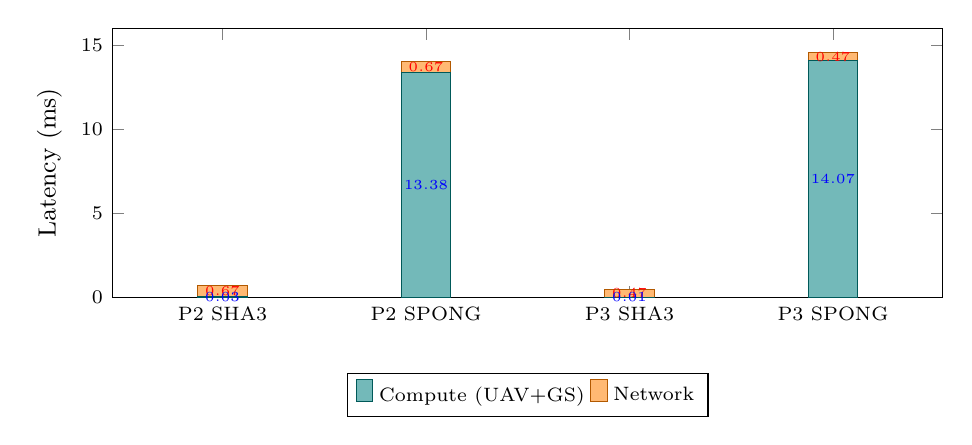
\begin{tikzpicture}
\begin{axis}[
    width=\columnwidth, height=5cm,
    ybar stacked, bar width=18pt,
    enlarge x limits=0.18,
    ymin=0, ymax=16,
    ylabel={Latency (ms)},
    symbolic x coords={A,B,C,D},
    xtick=data,
    xticklabels={P2 SHA3, P2 SPONG, P3 SHA3, P3 SPONG},
    legend style={at={(0.5,-0.28)}, anchor=north, legend columns=2,
                  font=\scriptsize},
    nodes near coords={\pgfmathprintnumber[fixed,precision=2]{\pgfplotspointmeta}},
    every node near coord/.append style={font=\tiny},
    x tick label style={font=\scriptsize},
    y tick label style={font=\scriptsize},
    label style={font=\small}
]
\addplot+[fill=teal!55, draw=teal!70!black]
  coordinates {(A,0.034) (B,13.379) (C,0.009) (D,14.069)};
\addplot+[fill=orange!55, draw=orange!70!black]
  coordinates {(A,0.665) (B,0.665) (C,0.467) (D,0.467)};
\legend{Compute (UAV+GS), Network}
\end{axis}
\end{tikzpicture}
\caption{Measured compute--network split per authentication.
SHA3 mode is network-bound ($95\%$ of latency); SPONGENT mode is
hash-bound ($95\%$).}
\label{fig:breakdown}
\end{figure}

Figure~\ref{fig:breakdown} visualizes the measured split.

\subsection{Total Swarm Authentication Time}
Table~\ref{tab:swarm} aggregates the time to fully authenticate
the ten-UAV swarm (ten UAV--GS exchanges plus $45$ peer pairs).

\begin{table}[t]
\centering
\caption{Total mutual authentication time for the 10-UAV swarm.}
\label{tab:swarm}
\begin{tabular}{@{}lrr@{}}
\toprule
\textbf{Step} & \textbf{SHA3} & \textbf{SPONGENT} \\
\midrule
Phase 2 ($10$ UAVs, ms)        & $6.99$       & $140.44$ \\
Phase 3 ($45$ pairs, ms)       & $21.42$      & $654.08$ \\
\midrule
\textbf{Grand total (ms)}      & $\mathbf{28.41}$ & $\mathbf{794.52}$ \\
\textbf{Overhead per pair (B)} & $\mathbf{279}$  & $\mathbf{279}$ \\
\bottomrule
\end{tabular}
\end{table}

In SHA3 mode the entire ten-UAV swarm achieves full mutual
authentication in under $30$~ms. In SPONGENT software mode the
total is $\sim$800~ms---still acceptable for a one-shot
initialization but uncompetitive with hardware acceleration
(\S\ref{sec:hwproj}).

\subsection{Per-UAV Storage}
\label{sec:storage}
Per-UAV storage scales as $S(N) = 560 + 40(N-1)$~bytes for an
$N$-UAV swarm: identity ($28$\,B), enrollment token ($20$\,B),
$12$~CRPs of helper data ($\sim$384\,B), and peer credentials for
$N{-}1$ peers ($40$\,B each). For $N{=}10$ this is $\sim 920$\,B per
UAV; for $N{=}100$ it is $\sim 4.5$\,KB. The GS, conversely, stores
$\sim 100\,N$\,bytes (CRPs plus credentials)---under $10$\,KB even
for a $100$-UAV swarm. By contrast, an RSA-2048 PKI deployment
requires $\sim 2$\,KB of per-UAV storage just for the local
certificate and CA root, before peer credentials.

\subsection{Comparison with Baselines}
\label{sec:compare}
Table~\ref{tab:compare} compares our Phase~2 latency against
representative baselines. Numbers for prior work are as reported on
ARM-class platforms; ours is on x86-64 (relative trends carry).

\begin{table}[t]
\centering
\caption{Phase 2 latency, overhead, and security feature comparison.}
\label{tab:compare}
\scriptsize
\setlength{\tabcolsep}{4pt}
\begin{tabular}{@{}lrrcc@{}}
\toprule
\textbf{Method} & \textbf{Latency} & \textbf{Bytes/pair}
& \textbf{P2P} & \textbf{No key} \\
\midrule
RSA-2048 PKI                                  & $\sim$15~ms       & $768$ & \cmark & \xmark \\
ECC-256 ECDSA                                 & $\sim$8~ms        & $384$ & \cmark & \xmark \\
PSK (AES-GCM)                                 & $\sim$0.5~ms      & $256$ & \cmark & \xmark \\
Gope \cite{puf_lightweight_uav}               & $10$--$50$~ms     & $512$ & \xmark & \cmark \\
Chatterjee \cite{puf_uav_cross_domain}        & $45$--$80$~ms     & $640$ & part.\ & \cmark \\
Khan \cite{puf_6g_uav}                        & $5$--$20$~ms      & $480$ & \xmark & \cmark \\
Bera \cite{peer2peer_auth}                    & $<\!1$~ms         & ---   & \cmark & \xmark \\
\textbf{This work (SHA3)}                     & $\mathbf{0.699}$~\textbf{ms} & $\mathbf{279}$ & \cmark & \cmark \\
\textbf{This work (SPONGENT, sw)}             & $\mathbf{14.04}$~\textbf{ms} & $\mathbf{279}$ & \cmark & \cmark \\
\bottomrule
\end{tabular}
\\\raggedright\scriptsize ``No key'' = no private/symmetric key
stored in NVM. Bytes/pair includes UAV--GS plus one peer exchange.
\normalsize
\end{table}

Our SHA3 mode is $11\times$ faster than ECC-256, $21\times$ faster
than RSA-2048, and $14$--$72\times$ faster than the surveyed PUF
baselines. Even our software SPONGENT mode is competitive with the
faster ARM-platform PUF schemes. Among all rows, only ours combines
direct peer-to-peer authentication with the no-stored-key property.

\subsection{Hardware Projection}
\label{sec:hwproj}
Published synthesis results~\cite{spongent_original,
lightweight_crypto_evaluation} report $5$--$10$~\textmu s per
SPONGENT-160 call on a $100$~MHz FPGA, versus our software
$\sim$890~\textmu s. SHA3 on FPGA is $1$--$2$~\textmu s, comparable
to its $0.4$~\textmu s software cost. Substituting hardware hash
latencies into the per-message breakdown
(Table~\ref{tab:phase2_break}) yields the projection in
Table~\ref{tab:hw}.

\begin{table}[t]
\centering
\caption{Projected total swarm authentication time on hardware.}
\label{tab:hw}
\begin{tabular}{@{}lrrr@{}}
\toprule
& \textbf{Software} & \textbf{FPGA} & \textbf{ASIC} \\
& (x86-64) & ($100$~MHz) & ($200$~MHz) \\
\midrule
SHA3 total (ms)      & $28.4$  & $28.7$ & $28.4$ \\
SPONGENT total (ms)  & $794.5$ & $33.0$ & $29.0$ \\
SW/HW gap            & ---     & $20\times$ & $25\times$ \\
\midrule
PUF+hash+BCH (GE)    & ---     & \multicolumn{2}{r}{$\sim$8{,}390 (SPONGENT)} \\
                     & ---     & \multicolumn{2}{r}{$\sim$44{,}200 (SHA3)} \\
\bottomrule
\end{tabular}
\end{table}

On hardware, the SHA3--SPONGENT latency gap collapses from
$20$--$30\times$ in software to $2$--$5\times$, while SPONGENT
requires $5\times$ less area. The complete PUF+SPONGENT+BCH security
stack fits in $\sim$8{,}390~GE---smaller than a single ARM Cortex-M0
core, enabling integration as a dedicated security co-processor on
the UAV flight controller.


% ========================================================================
\section{Security Analysis and Discussion}
\label{sec:security}

\textbf{Mutual authentication (Phase 2).} An adversary forging $M_3$
must produce a valid hash of $R^{\mathrm{masked}} \| \mathrm{SK}_i$
where $\mathrm{SK}_i = h(R \| N_1 \| N_2 \| T_1)$. Since $R$ is not
derivable from publicly visible helper data (helper-data
security~\cite{helper_data_masking}) and is never transmitted in
clear, hash pre-image resistance bounds the forgery probability by
$2^{-160}$. Conversely, $\beta_1$ in $M_2$ binds the GS to a CRP
challenge known only to the GS database; forging it requires
database compromise.

\textbf{Replay resistance.} Every message carries a fresh
$128$-bit nonce and a $32$-bit timestamp validated within a
$\Delta T_{\max}{=}5$~s window. CRPs are consumed on successful
Phase~2, so replay of $M_3$ against a fresh challenge fails by
construction.

\textbf{Peer authentication (Phase 3).} Possession of $\mathrm{Cred}$
is gated by Phase~2 success, hence by PUF possession. The token chain
$(\tau_1,\tau_2,\tau_3)$ binds both nonces and both identities to
$\mathrm{Cred}$; an adversary without $\mathrm{Cred}$ cannot produce
a valid $\tau$ except with probability $2^{-160}$. We acknowledge
that this is a coarser root of trust than per-pair PUF rekeying: a
captured UAV's $\mathrm{Cred}$ permits peer impersonation until
swarm re-enrollment. Mitigation via $\mathrm{Cred}$ rotation on a
re-enrollment cycle bounds this attack window; per-pair PUF-rooted
peer authentication is available as a ``high-security mode''
extension at the cost of an additional Phase~2-like exchange per
peer pair.

\textbf{Physical capture resistance.} A captured UAV's NVM exposes
only its TID and (transiently) $\mathrm{Cred}$. The captured UAV
cannot impersonate any other UAV in a fresh Phase~2 because PUF
unclonability binds each $R_j$ to UAV~$j$'s physical PUF. Invasive
probing destroys the PUF response.

\textbf{Limitations.} (i) The OMNeT++ delay model omits MAC-layer
contention; real $802.11$ deployments would add $1$--$10$~ms per
message from CSMA/CA, ACKs, and retransmissions. This overhead is
the same for all authentication protocols, so the relative ranking
is preserved. (ii) Our SPONGENT software variant uses a compact
bit-permutation; the absolute SPONGENT software cost is
representative rather than authoritative, but the hardware
projection (where the permutation is zero-cost wire routing) is
unaffected. (iii) The Arbiter PUF is simulated, not measured on
silicon; FPGA prototyping is the natural next step.


% ========================================================================
\section{Conclusion}
\label{sec:conclusion}

We presented and evaluated a four-phase PUF-based authentication
protocol for UAV swarms with a complete OMNeT++~6.3 reference
implementation and dual hash-mode characterization. Measured
end-to-end Phase~2 latency is $0.699$~ms (SHA3) / $14.044$~ms
(SPONGENT), and Phase~3 per-pair latency is $0.476$~ms /
$14.535$~ms, with $100\%$ success across all ten UAV--GS exchanges
and all $45$ peer pairs and $279$~bytes total overhead per UAV pair.
Network delay dominates SHA3-mode latency ($95\%$);
BCH(255,131,18) absorbs $3\%$ PUF noise with $4.7\times$ margin;
and FPGA projection shows the SHA3--SPONGENT gap collapses from
$20$--$30\times$ in software to $2$--$5\times$, making SPONGENT the
natural choice for ASIC-integrated UAV authentication at
$\sim$8{,}390~GE total. Future work includes Xilinx Artix-7 FPGA
prototyping, MAVLink~2.0 integration, formal symbolic verification
with ProVerif/Tamarin, $50$--$100$-UAV scalability studies, and
adversarial evaluation (jamming, Sybil, replay).


% ========================================================================
\balance
\begin{thebibliography}{99}
\bibitem{securing_uav_fanet} A.~Mukherjee \textit{et al.},
``Securing UAV flying ad hoc wireless networks: Authentication
development for robust communications,'' \emph{IEEE Access},
vol.~12, pp.~1--15, 2024.

\bibitem{puf_lightweight_uav} P.~Gope and B.~Sikdar, ``A PUF-based
lightweight authentication and key agreement protocol for smart UAV
networks,'' \emph{IET Commun.}, vol.~16, no.~18, pp.~2136--2148,
2022.

\bibitem{peer2peer_auth} T.~Bera, S.~Das, and A.~K.~Das,
``Secure and efficient peer-to-peer authentication-attestation
protocol for UAV networks,'' in \emph{Proc.\ IEEE INFOCOM Wkshps.},
2023, pp.~1--6.

\bibitem{puf_uav_cross_domain} B.~Li \textit{et al.}, ``PUF-based
secure and efficient anonymous authentication protocol for UAV
towards cross-domain environments,'' \emph{IEEE Trans.\ Veh.\
Technol.}, vol.~72, no.~9, pp.~12101--12115, 2023.

\bibitem{puf_6g_uav} S.~Khan \textit{et al.}, ``A provably secure
and lightweight PUF-based authentication scheme for 6G-enabled UAV
networks,'' \emph{IEEE Internet Things J.}, vol.~11, no.~5,
pp.~8532--8543, 2024.

\bibitem{puf_overview} A.~Alkatheiri, Y.~G.~Alghamdi, and
S.~U.~Jan, ``Review of physically unclonable functions (PUFs):
Structures, models, and algorithms,'' \emph{Frontiers Electronics},
vol.~4, p.~1123456, 2023.

\bibitem{arbiter_puf_iot} L.~Xu \textit{et al.}, ``An enhanced
event-based dynamic authentication protocol leveraging Arbiter PUF
for IoT devices,'' \emph{IEEE Internet Things J.}, vol.~10, no.~18,
pp.~16123--16135, 2023.

\bibitem{spongent_original} A.~Bogdanov \textit{et al.},
``SPONGENT: A lightweight hash function,'' in \emph{Proc.\ CHES},
LNCS 6917, Springer, 2011, pp.~312--325.

\bibitem{sha3_standard} NIST, \emph{SHA-3 Standard:
Permutation-Based Hash and Extendable-Output Functions},
FIPS PUB~202, Aug.~2015.

\bibitem{lightweight_crypto_evaluation} T.~Eisenbarth \textit{et
al.}, ``Design and evaluation of lightweight cryptographic
primitives for constrained devices,'' \emph{J.\ Cryptographic
Eng.}, vol.~12, no.~3, pp.~245--260, 2022.

\bibitem{bch_puf_extraction} J.~Delvaux \textit{et al.},
``Cryptographic key generation from PUF data using efficient fuzzy
extractors,'' \emph{IEEE Trans.\ Inf.\ Forensics Security}, vol.~15,
pp.~2025--2038, 2020.

\bibitem{helper_data_masking} R.~Maes, ``Helper data masking for
physically unclonable function-based key generation,'' Cryptology
ePrint Archive, Report 2019/688, 2019.

\bibitem{sram_puf_bch} L.~Zhang \textit{et al.}, ``SRAM-PUF key
extraction method and performance analysis based on RS and BCH
codes,'' \emph{Electronics}, vol.~12, no.~4, p.~1012, 2023.

\bibitem{dolev_yao} D.~Dolev and A.~C.~Yao, ``On the security of
public key protocols,'' \emph{IEEE Trans.\ Inf.\ Theory}, vol.~29,
no.~2, pp.~198--208, Mar.~1983.

\bibitem{puf_iot_strong_adversary} U.~Chatterjee, R.~S.~Chakraborty,
and D.~Mukhopadhyay, ``PUF-based authentication in IoT against
strong physical adversary,'' in \emph{Proc.\ IEEE DATE}, 2022,
pp.~1--6.

\bibitem{puf_mitm_dos} S.~Dey and M.~Hossain, ``MITM- and
DoS-resistant PUF authentication for industrial WSNs via
sensor-initiated registration,'' \emph{IEEE Internet Things J.},
vol.~10, no.~22, pp.~19740--19753, 2023.

\bibitem{puf_secure_design} M.~Hassan \textit{et al.}, ``Designing
secure PUF-based authentication protocols for IoT devices,''
\emph{Sci.\ Rep.}, vol.~13, p.~21856, 2023.

\bibitem{puf_uav_security_analysis} S.~Banerjee \textit{et al.},
``On the security of the novel authentication scheme for UAV--GS
communication,'' in \emph{Proc.\ IEEE WiMob}, 2023, pp.~1--6.

\bibitem{puf_key_exchange} R.~Aman \textit{et al.}, ``PUF-based
lightweight authentication and key exchange protocol for IoT,'' in
\emph{Proc.\ IEEE GLOBECOM}, 2022, pp.~1--6.

\bibitem{omnetpp} A.~Varga and R.~Hornig, ``An overview of the
OMNeT++ simulation environment,'' in \emph{Proc.\ ICST SIMUTools},
2008, art.~60.

\bibitem{keccak_team} G.~Bertoni, J.~Daemen, M.~Peeters, and
G.~Van~Assche, ``The Keccak reference, version 3.0,'' Jan.~2011.
\end{thebibliography}

\end{document}
